
\emph{Deep Learning} (DL), também conhecido como Aprendizado Profundo, é uma subárea específica de ML que enfatiza o aprendizado através de sucessivas camadas de representações cada vez mais significativas dos dados submetidos. Estas representações são quase sempre obtidas atráves de redes neurais profundas \cite{chollet}. De acordo com Heaton, qualquer RNA com mais de duas camadas ocultas é, em sua essência, considerada profunda \cite{heaton}. O DL tem obtido um êxito incrível em endereçar problemas de visão computacional e processamento de linguagem natural. Estes algoritmos não só ultrapassaram outras variedades de algoritmos de ML, como também pleiteam a eficácia na classificação alcançada por seres humanos \cite{buduma}.

Os motivos para o corrente sucesso do DL podem ser exemplificados pela grande quantidade de dados disponíveis -- como a base de dados \emph{ImageNet}, organizada conforme a hierarquia \emph{WordNet} e que disponibiliza imagens para pesquisadores ao redor do mundo \cite{imagenet} -- e o custo relativamente baixo de Unidades de Processamento Gráfico (GPUs), que são utilizadas para uma computação numérica muito mais eficiente. Grandes companhias do ramo tecnológico utilizam técnicas de DL diariamente para a análise de enormes quantidades de dados. Entretanto, esta especiliadade não é mais limitada somente ao domínio acadêmico e industrial, ela tornou-se parte integrante da produção de softwares modernos disponibilizados aos consumidores \cite{gulli}.

O DL reúne um conjunto de técnicas e modelos que podem ser aplicados a tarefas de aprendizado supervisionado e não-supervisionado, nas quais as redes neurais convolucionais se destacam expressivamente. A próxima seção descreve os pontos principais relacionados a este tipo de RNA.

\subsubsection{Redes Neurais Convolucionais}
\label{subsubsec:cnns}

As \emph{Redes Neurais Convolucionais} (CNNs, do inglês \emph{Convolutional Neural Networks}) são uma categoria de redes neurais profundas, \emph{feedforward}, que comprovaram ser extremamente bem-sucedidas no ramo de visão computacional \cite{khan}. O termo denominado a estas redes, vem do seu aproveitamento da operação matemática chamada convolução, um tipo especializado de operação linear \cite{goodfellow}.

% Convolução
A \emph{convolução} é uma operação que consiste na soma dos produtos de toda a extensão de duas entradas em função de um deslocamento. Sendo assim, a convolução $s(t)$ de duas entradas $x_1(t)$ e $x_2(t)$ é uma função representada simbolicamente por $s(t) = x_1(t) * x_2(t)$ e definidade conforme a Equação \ref{eq:conv} \cite{lathi}.

\begin{equation}
  \label{eq:conv}
  s(t) = x_1(t) * x_2(t) = \int_{-\infty}^{\infty} x_1(\tau)x_2(t - \tau)d\tau
\end{equation}

Nas aplicações de ML, a função $x_1(t)$ é chamada de \emph{input}, a função $x_2(t)$ é o \emph{filtro}, também conhecido como \emph{kernel}, e a saída $s(t)$ consiste no \emph{mapa de características}, gerado pela convolução. O \emph{input} é geralmente uma matriz multidimensional de dados de entrada e o filtro é uma matriz multidimensional de de parâmetros que são ajustados pelo algoritmo de aprendizado. Uma matriz multidimensional no contexto de ML é comumente referenciada como \emph{tensor} \cite{goodfellow}.

As camadas convolucionais são responsáveis por aplicar as operações de convolução. Tomando como exemplo um problema de reconhecimento de padrões em uma imagem, cada camada é responsável por desenvolver os atributos detectados nas camadas anteriores - de linhas, a contornos, a formatos, até construir um objeto por completo. Esse processo pode ser visualizado na Figura \ref{fig:camadas-convolucionais}. Nestas camadas os mapas de características são capturados, e nestes consistem os pesos da rede que são responsáveis por identificar onde são encontrados os atributos na imagem original \cite{buduma}.

\begin{figure}[h!]
\centering
\caption{Processo reproduzido pelas camadas convolucionais de uma CNN, aplicado a um problema de classificação de imagens. Fonte: \cite{khan}.}
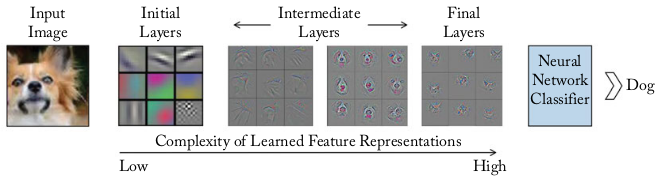
\includegraphics[width=0.9\textwidth]{imgs/camadas-convolucionais}
\label{fig:camadas-convolucionais}
\end{figure}


% Pooling
Uma camada de \emph{pooling} em uma CNN opera em blocos do mapa de características e combina seus atributos através da operação de \emph{max pooling} ou \emph{average pooling}. Esse bloco é deslizado através do mapa de características com um passo definido como \emph{stride}. A operação de \emph{max pooling} retorna o valor máximo dos dados em uma área retangular. Enquanto a operação de \emph{average pooling}, realiza o mesmo processo do \emph{max pooling}, mas com a média dos valores. O propósito da camada de \emph{pooling} é, além de diminuir a quantidade de amostras no mapa de características, ajudar a sua representação a se tornar invariante a pequenas mudanças nos dados de entrada \cite{khan, goodfellow}. Uma visualização detalhada dessa operação é demonstrada na Figura \ref{fig:pooling}.

\begin{figure}[h!]
  \centering
  \caption{Visualização da operação de \emph{max pooling} considerando uma região de 2 x 2 com um \emph{stride} igual a 1. Fonte: \cite{khan}.}
  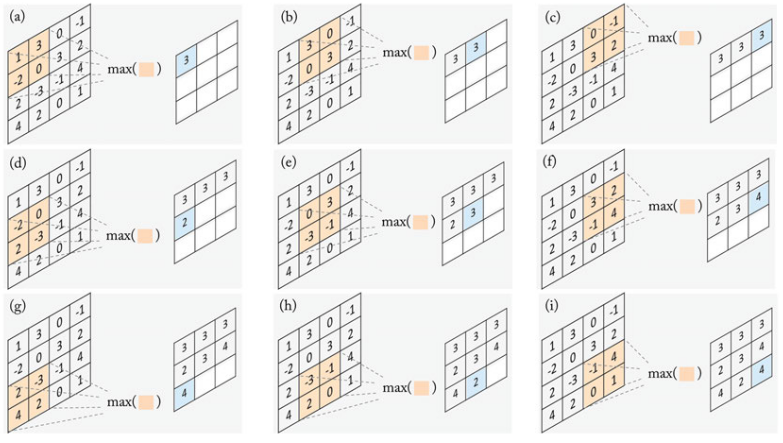
\includegraphics[width=0.8\textwidth]{imgs/pooling}
  \label{fig:pooling}
\end{figure}

% Fully connected layers, camada de saída??

As \emph{Fully Connected Layers}, ou camadas completamente conectadas, considera um conjunto de neurônios completamente conecetados entre si, sendo comumente encontradas no final de uma CNN. Possui a capacidade de separar as variações de classificação que serão retornadas na saída, resumindo os resultados dos vários mapas de características produzidos pela rede \cite{gulli}.

% Dropout (Pegar imagens sobre Dropout na pagina favoritada)


\begin{figure}[h!]
  \centering
  \caption{A relação entre a visão humana, visão computacional, ML, DL e CNNs. Adaptado de: \cite{khan}.}
  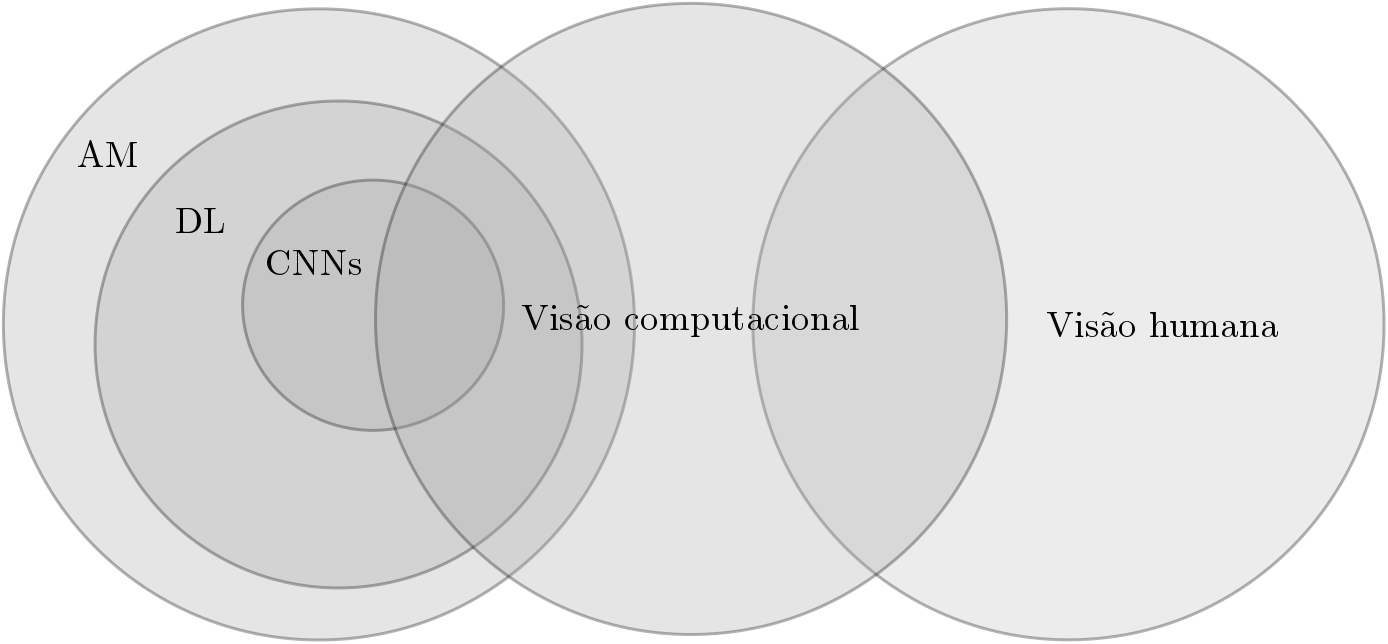
\includegraphics[height=4cm]{imgs/areas-ia}
  \label{fig:areas-ia}
\end{figure}
\todo{Inserir essa imagem no contexto.}
% Arquiteturas canônicas


\subsubsection{Arquiteturas canônicas de Redes Neurais Convolucionais}
\label{subsubsec:arq-cnns}
